


\chapter[Structure]{\href{https://ieeexplore.ieee.org/abstract/document/9116004}{\color{blue}Structure}}

\textbf{Appeared as:}\\
S.~Kriegman et al.,
Scalable sim-to-real transfer of soft robot designs,
\textit{Proceedings of the IEEE International Conference on Soft Robotics (RoboSoft)} (2020).


\chapter[Shape]{\href{https://dl.acm.org/doi/abs/10.1145/3071178.3071296}{\color{blue}Shape}}

\textbf{Appeared as:}\\
S.~Kriegman, et al., A minimal developmental model can increase evolvability in soft robots. \textit{Proceedings of the Genetic and Evolutionary Computation Conference} (2017).


\chapter[Shape and Configuration]{\href{https://www.nature.com/articles/s41598-018-31868-7}{\color{blue}Shape and Configuration}}

\textbf{Appeared as:}\\
S.~Kriegman, et al., How morphological development can guide evolution. \textit{Scientific reports} \textbf{8}, 13934 (2018).


\chapter[Material, Structure, Configuration]{\href{https://arxiv.org/abs/1804.02257}{\color{blue}Material, Structure, Configuration}}

\textbf{Appeared as:}\\
S.~Kriegman et al., Interoceptive robustness through environment-mediated morphological development. \textit{Proceedings of the Genetic and Evolutionary Computation Conference} (2018).


\chapter[Structure, Shape, Configuration]{\href{http://www.roboticsproceedings.org/rss15/p28.html}{\color{blue}Structure, Shape, Configuration}}

\textbf{Appeared as:}\\
S.~Kriegman et al., Automated shapeshifting for function recovery in damaged robots. \textit{Proceedings of Robotics: Science and Systems} (2019).


\chapter[Xenobots: Material, Structure, Shape, Configuration]{\href{https://www.pnas.org/content/117/4/1853}{\color{blue}Xenobots: \\ {\LARGE Material, Structure, Shape, Configuration}}}

\textbf{Appeared as:}\\
S.~Kriegman et al., A scalable pipeline for designing reconfigurable organisms. 
\textit{Proceedings of the National Academy of Sciences (PNAS)} (2020).



%%%%%%%%%%%%%%%%%%%%%%%%%%%%%%%%%%%%%%%%%%%%%%%%%%%%%%%%


\chapter{Argument}


\section{Pr\'{e}cis of the Thesis}

\textsc{In Chapter 1,}
a history of 
evolved robots 
and protean machines was provided
to situate the contributions of the present thesis in the literature.
Two motivating observations were made at the very beginning:
(1) organisms are autonomous adaptive systems, robots are not;
(2) organisms are exceedingly protean systems, robots are not.
This thesis is at heart about closing this robot-organism gap by means of increasingly protean machines.
Designing such systems is both operationally and conceptually challenging.
Perhaps because of the former reason, despite early investigations by Pask and Beer (and a mini-Enlightenment at Sussex University in the 1990s), protean machines remain a neglected research program.



To demonstrate 
the value of incorporating increasingly more morphological plasticity in robots,
I started with

the evolution of ontogenetically static structure

the evolution of ballistic ontogenetic shape change

the evolution of ballistic ontogenetic change to resting shape and configuration osculations occurring and interacting on two timescales.

the evolution of material properties (stiffness) in response to environmental signals (stress, pressure)


the evolution of configuration alternatives in a fixed structure; increasingly deeper mechanical amputations to that structure, each time automatically developing a new shape the recovered function without changing the controller.

finally, the design and manufacture of novel organisms

The following sections summarize each of these 
% preceding 
% succeeding
chapters in turn.


\section{Sim-to-Real for Structure}
% Soft Robot Blocks

\textsc{In Chapter 2,}
a low cost, open source, and modular soft robot design and construction kit was introduced and used to
transfer an order of magnitude more robot designs from simulation to reality than any other method to date.

\subsection{Protean Capacity}

\begin{itemize}
    \item \textit{Phylogenic change}: structure, material distribution.
    \item \textit{Ontogenic change}: configuration.
\end{itemize}

\subsection{Realization}
% Realization, Concretization, Actualization

\begin{itemize}
    \item \textit{Material}: passive and pneumatically-actuated silicone voxels (cubic bladders).
    \item \textit{Structure}: number, placement and kind of voxels.
    \item \textit{Shape} [fixed]: atmospheric pressure (cubes).
    \item \textit{Configuration}: pressure oscillation of all active voxels in unison (expansion, compression back to cube, hold at cube, repeat).
\end{itemize}



\subsection{Contribution}



There is little to no data on the simulation-reality gap for soft robots.
By transferring a diversity of soft robot designs from simulation to reality, the reality gap was measured as a function of morphology given a static control policy.
Under one measure (net displacement) the reality gap appeared rather small, but under another (velocity) the gap was much wider.
This illuminated the fact that there are reality gaps rather than a single gap.
This suggests that, if structure is allowed to vary, automated design can be used as a filter to discover morphologies which reduce the gap before attempting to cross it with controller optimization.

The kit's affordability, safety, speed, and simplicity effectively lower the barrier of entry to soft robotics for non-experts.
Such a tool is posed to generate increasingly more, and more reproducible, data about the design of protean machines.
In the age of covid, a do-it-yourself-at-home soft robot kit 
is particularly appealing and has been adopted by four soft robotics research labs thus far.



\section{Ballistic Development}


\textsc{In Chapter 3,}
a minimal yet embodied model of development: 
the shape of the
robot changes over its lifetime, yet development is not influenced
by the environment. 
It was shown that even this simple developmental
model confers evolvability because it allows evolution to sweep over a larger range of body plans than an equivalent non-developmental system, and subsequent heterochronic mutations
`lock in' this body plan in more morphologically-static descendants.


\subsection{Protean Capacity}

\begin{itemize}
    \item \textit{Phylogenic change}: shape alternatives.
    \item \textit{Ontogenic change}: shape, configuration.
\end{itemize}


\subsection[Concretization]{Concretization\footnote{This particular capacity for morphological change was concretely demonstrated in a computational yet embodied model (in silico), however it was not \textit{realized}: no physical robot was used during hypothesis testing.}}

\begin{itemize}
    \item \textit{Material} [fixed]: actuated voxels (1 to 6 elastic beams).
    \item \textit{Structure} [fixed]: a 4-by-4-by-3 block of voxels (48 voxels; 108 elastic beams).
    \item \textit{Shape}: evolved initial and final sets of rest volumes (resting beam lengths) for each voxel; linear ontogenetic shape change between sets.
    \item \textit{Configuration} [fixed]: voxel length oscillation, all voxels in unison (expansion/contraction according to sine wave with frequency 4 Hz).
\end{itemize}


\subsection{Contribution}


Protean body plans introduce smaller and thus safer mutations \cite{lehman2018safe}, whose behavioral deflection manifests temporarily during operation, rather than permanently from deployment (chapter 3).
Evolution can then lengthen the time intervals containing superior traits and reduce the intervals of inferior traits.
This allows evolution to surgically revise morphology with a pair of tweezers, if you will, rather than a sledgehammer.


% In this chapter I introduced a minimal yet embodied model of development in order to isolate the effect of morphological change in ontogenetic time,
% without the confounding effects of environmental mediation.
% Even this simple developmental model naturally provides
% a continuum in terms of the magnitude of mutational phenotypic impact,
% from the very large (caused by early-in-life developmental mutations) 
% to the very small (caused by late-in-life mutations). 
% It was predicted that,
% because of this, such a developmental system will be more evolvable than an equivalent non-developmental system because the latter lacks this inherent spectrum in the magnitude of mutational impacts.




\section{Differential Canalization}

\textsc{In Chapter 4,}
a previously unknown phenomenon when embodied agents are allowed to develop and evolve: Evolution discovers body plans robust to control changes, these body plans become genetically assimilated, yet controllers for these agents are not assimilated. 
This allows evolution to continue climbing fitness gradients by tinkering with the developmental programs for controllers within these permissive body plans. 
This exposes a previously unknown detail about the Baldwin effect: instead of all useful traits becoming genetically assimilated, only traits that render the agent robust to changes in other traits become assimilated. 
We refer to this as \textit{differential canalization}.


\subsection{Protean Capacity}

\begin{itemize}
    \item \textit{Phylogenic change}: shape alternatives, configuration alternatives.
    \item \textit{Ontogenic change}: shape, configuration.
\end{itemize}


\subsection{Concretization}

\begin{itemize}
    \item \textit{Material} [fixed]: same as chapter 3.
    \item \textit{Structure} [fixed]: same as chapter 3.
    \item \textit{Shape}: same as chapter 3.
    \item \textit{Configuration}: voxel length oscillation phase shifted from a central pattern generator (sine wave with frequency 4 Hz).
    Evolved initial and final of phase offsets for each voxel; linear ontogenetic phase-offset change between sets.
\end{itemize}



% The same
% a 4-by-4-by-3 voxel
% structure from chapter 3 was used endowed with more configuration plasticity in chapter 4.
% Instead of uniform expansion/contraction throughout the structure,
% phase-offsets were introduced to locally vary excitation relative to a central pattern generator.
% Both resting shape and the phase-offsets of configuration oscillations changed ballistically and the starting and ending points were evolved.


\subsection{Contribution}

gradients in morphospace

Protean body plans smooth the search space evolution operates in via the Baldwin effect (chapters 3 and 4).
This effect is outlined in Figs.~\ref{fig:baldwin2d} and \ref{fig:baldwin3d}.
In brief, the flexibility of a protean feature
(e.g.~skin thickness) allows evolution to sweep through design space along a line of development rather than sampling a single point.
Development can then be incrementally canalized about a good static setting (e.g.~calluses).
This gradual homing-in process is hastened by natural selection,
and eventually supplanted by the genetic determination of the feature 
% which in previous generations needed to be rediscovered by development. 
(e.g.~embryonic calluses).
% that in previous generations was protean.
%  that would otherwise be need to be earned through interaction with the environment
This well-studied phenomenon is revisited with a twist:
physically embodied robots, rather than an abstract control system.
This distinction is important because it grounds hypotheses in the constraints and opportunities afforded by the physical world.


Protean body plans promote (the canalization of) permissive body plans robust to control changes (chapter 4).
It is much easier to train a control policy within a permissive body. 
% Evolution discovers body plans robust to control changes, these body plans become genetically assimilated, yet controllers for these agents are not assimilated.
This exposed a previously unknown detail about the Baldwin effect: instead of all useful traits becoming genetically assimilated, only traits that render the agent robust to changes in other traits become assimilated. 
% This exposed the previously unknown phenomenon of differential canalization reported here.
I refer to this as \textit{differential canalization}.

% \noindent
% In these experiments, the intersection of two time scales---slow linear development and rapid oscillatory actuation, as from a central pattern generator---generates positive and negative feedback in terms of instantaneous velocity: the robot speeds up and slows down during various points in its lifetime.
% Prior to canalization, unless all of the phenotypes swept over by an individual in development keep the robot motionless, there will be intervals of relatively superior and inferior performance.
% Evolution can thus improve overall fitness in a descendant by lengthening the time intervals containing superior phenotypes and reducing the intervals of inferior phenotypes. However, this is only possible if such mutations exist.

% We have found here that such mutations do exist in cases where evolutionary changes
% to one trait do not disrupt the successful behavior contributed
% by other traits.
% For example,
% robots that exhibited the locally optimal trotting behavior 
% exhibited a tight coupling between morphology and control, and thus evolution was 
% unable to canalize development in either one, since mutations to one subsystem 
% tended to disrupt the other.
% Brief ontogenetic periods of rolling behavior, 
% on the other hand, could be temporally extended by evolution through canalization of the morphology alone, 
% since these morphologies are generally robust to the pattern of actuation.
% The key observation here is that only phenotypic traits that render the agent robust to changes in other traits become assimilated, a phenomenon we term differential canalization. 

% This insight was exposed by modeling the development of simulated robots as they interacted with a physically realistic environment.
% Differential canalization may be possible in disembodied agents as well, 
% if they conform to appropriate conditions described in the chapter.

% This finding of differential canalization has important implications for the evolutionary design of artificial and embodied agents such as robots.
% Computational and engineered systems generally maintain a fixed form as they behave and are evaluated.
% However, these systems are also extremely brittle when confronted with slight changes in their internal structure, such as damage, 
% or in their external environment such as moving onto a new terrain
% \cite{french1999catastrophic,
% carlson2005ugvs,
% bongard2006resilient}.
% Indeed, a perennial problem in robotics and AI is finding general solutions which perform well in novel environments 
% \cite{koos2013transferability,
% nguyen2015deep
% }.
% Our results demonstrate how incorporating morphological development in the optimization of robots can reveal, through differential canalization, characters which are robust to internal changes.
% Robots that are robust to internal changes in their controllers may also be robust to external changes in their environment \cite{bongard2011morphological}.
% Thus, allowing robots to change their structure as they behave might facilitate evolutionary improvement of their descendants, even if these robots will be deployed with static phenotypes or in relatively unchanging environments.

% These results are particularly important for the nascent field of soft robotics in which engineers cannot as easily presuppose a robot's body plan and optimize controllers for it because designing such machines manually is unintuitive
% \cite{lipson2014challenges, pfeifer2012challenges}.
% Our approach addresses this challenge, because differential canalization provides a mechanism whereby static yet robust soft robot morphologies may be automatically discovered using evolutionary algorithms for a given task environment.
% Furthermore, future soft robots could potentially alter their shape to best match the current task by selecting from previously trained and canalized forms.
% This change might occur pneumatically, as in \citet{shepherd2011multigait}, or it could modulate other material properties such as stiffness (e.g.~using a muscular hydrostat).

% We have shown that 
% for canalization to occur in our developmental model, some form of paedomorphosis must also occur. However, there are at least two distinct methods by which such heterochrony can proceed: progenesis and neoteny.
% Progenesis 
% % |the acceleration of developmental processes such that adult traits of ancestors are realized earlier in juvenile stages of descendants| 
% could occur through mutations which move initial parameter values $(\ell,\, \phi)$ toward their final values $(\ell^*,\, \phi^*)$.
% Neoteny 
% % |the retention of juvenile traits into the adult form as a result of retardation of development| 
% could instead occur through mutations which move final values $(\ell^*,\, \phi^*)$ toward their initial values $(\ell,\, \phi)$.
% Although a superior phenotype can materialize anywhere along the ontogenetic timeline, late onset mutations are less likely to be deleterious than early onset mutations.
% This is because our developmental model is linear in terms of process, and interfering with any step affects all temporally-downstream steps. 
% Since the probability of a mutation being beneficial is inversely proportional to its phenotypic magnitude, mutational changes in the terminal stages of development require the smallest change to the developmental program.
% Hence, late-onset discoveries of superior traits are more likely to occur without breaking functionality at other points in ontogeny, and these traits can become canalized by evolution through progenesis: mutations which reduce the amount of ontogenetic time prior to realizing the superior trait (by moving $\ell \rightarrow \ell^*$ and/or $\phi \rightarrow \phi^*$). 
% Indeed progenesis was observed most often in our trials: late onset mutations which transform a walking robot into a rolling one are discovered by the evolutionary process, and are then moved back toward the birth of the robots'
% descendants through subsequent mutations.

% Finally, we would like to note the observed phenomenon of \textit{increased} 
% % phenotypic 
% % ballistic
% plasticity prior to genetic assimilation.
% Models of the Baldwin effect usually assume that phenotypic plasticity itself does not evolve, although it has been shown how major changes in the environment can select for increased plasticity in a character that is initially canalized \cite{lande2009adaptation}.
% In our experiments however, there is no environmental change.
% There is also a related concept known as `sensitive periods' of development in which an organism's phenotype is more responsive to experience 
% \cite{bateson1979sensitive}.
% Despite great interest in sensitive periods, the adaptive reasons why they have evolved are unclear \cite{Fawcett2015}.
% In our model, increasing the amount of morphological development increases the chance of capturing an advantageous static phenotype, which can then be canalized, once found.
% However, a phenotype will not realize the globally optimal solution by simply maximizing development.
% This would merely lengthen the \textit{line} on which development unfolds in phenotypic hyperspace ($n$-dimensional real space).


% The developmental model described herein is intentionally minimalistic in order to isolate the effect of morphological and neurological change in the evolutionary search for embodied agents.
% The simplifying assumptions necessary to do so make it difficult to assess the biological implications.
% For example, we model development as an open loop process 
% and thus ignore environmental queues and sensory feedback 
% \cite{Moczekrspb20110971,snell2013overview}.
% We also disregard the costs and constraints of phenotypic plasticity 
% \cite{snell2012selective,murren2015constraints}. 
% By removing these confounding factors, we hope these results will help generate novel hypotheses about morphological development, heterochrony, modularity and evolvability in biological systems.




\section{Environment-Mediated Development}

\textsc{In Chapter 5,}
we show robustness can be achieved by evolving the 
geometry of soft robots, their control systems, and how
their material properties develop in response to one particular interoceptive stimulus (engineering stress) during their lifetimes.
By doing so we realized robots that were equally fit but more robust to  extreme material defects (such as might occur during fabrication or by damage thereafter) than robots that did not develop during their lifetimes, or developed in response to a different interoceptive stimulus (pressure).
This suggests that the interplay between changes
in the containing systems
of agents (body plan and/or neural architecture)
at different temporal scales (evolutionary
and developmental) along different modalities
(geometry, material properties, synaptic weights)
and in response to different signals (interoceptive
and external perception) all
dictate those agents' abilities to evolve or 
learn capable and robust strategies.


\subsection{Protean Capacity}

\begin{itemize}
    \item \textit{Phylogenic change}: structure; material alternatives, configuration alternatives.
    \item \textit{Ontogenic change}: material, configuration.
\end{itemize}


\subsection{Concretization}


\begin{itemize}
    \item \textit{Material} [ill-specified]: dense voxels with evolved initial elasticity (Young's modulus between $10^4$ and $10^{10}$ MPa), and evolved rate of ontogenetic softening/stiffening in response to engineering stress / pressure.
    \item \textit{Structure}: evolved number and placement within a 10-by-10-by-10 workspace.
    \item \textit{Shape} [fixed]: cubes.
    \item \textit{Configuration}: voxel length oscillation phase shifted from a central pattern generator (sine wave with frequency 5 Hz).
\end{itemize}


% The constraint in chapters 2 to 4 of well-specified material were lifted in chapter 5.
% As in chapter 2,
% structure is free to vary but shape was not.
% However, a much larger, 10-by-10-by-10 workspace was used.
% The contribution of this chapter is that,
% instead of no development (chapter 2) or ballistic development (chapters 3 and 4),
% development is driven by environmental signals (stress and pressure).


\subsection{Contribution}

Protean body plans foster ``zero-shot'' generalization (on the very first try, without adjustment) to fabrication errors (chapter 5).
The amount of generalization in canalized (previously protean but now morphologically-static) machines was found to depend on the kinds of interoceptive signals used to guide their morphological change during optimization.

% \noindent
% % Initial exploration in closing the developmental feedback loop with as little additional machinery as possible to determine when and how such added complexity increases evolvability and robustness.
% Building systems that are robust in the face of changing environmental conditions is a grand challenge in robotics and AI.
% The brittleness of current systems is exemplified by the growing literature on adversarial examples
% \citep{szegedy2013intriguing,
% nguyen2015deep,
% athalye2017synthesizing}, 
% and the fact that almost all practical robots are confined to the perfectly flat floors they clean, or the hermetic factories built around their work.
% Robustness is not unknown in human-engineered systems, but it is relatively rare; in nature it is everywhere, and one of the reasons is that in nature organisms develop: 
% They constantly change not just their cognitive architectures but the morphologies that contain them and mediate with the external world.

% It has been shown for rigid robots \citep{bongard2011morphological}
% that morphological development can in some cases increase robustness since it exposes evolution to 
% richer sensory information: the robot must maintain locomotion while changing its body. 
% Soft robots have much greater potential in this domain:
% If soft, there are more ways that morphology can change, so by definition the increase
% in breadth in sensorimotor experiment induced by development will be even greater than that
% for developing yet rigid machines.
% Toward this goal, by allowing material stiffness to be plastic, we have here 
% investigated a heretofore unexplored dimension of morphological change (stiffness) not available
% to rigid robots.

% Advances in materials science and 3D printing promise new engineered systems{\textemdash} protean machines{\textemdash}that may continuously morph in response to changing environmental signals.
% Simply put, if a robot always changes its strategy along many morphological and neural modalities, 
% it is more difficult to fool with a static adversarial example or a new task environment.
% Little to no analysis has been conducted, however, into how such systems should respond to environmental stimuli in order to adapt their functions in the face of changing environmental conditions.

% In initiating such a study here, we have shown that it is not just a matter of reacting to \textit{any} stimulus: different types of developmental feedback loops elicit different \textit{evolved} properties.
% We observed that if one modality (stiffness) responds to one particular internal signal (engineering stress) but not another (pressure), robots evolved structure that  intrinsically buffered large deviations from their expected material properties.

% % Pressure and stress have very different mechanical load signatures, and so too were the developmental reactions they stimulated.
% Pressure and stress bear distinct mechanical load signatures which in turn stimulated very different developmental reactions.
% Intriguingly, increased robustness was correlated with increased canalization: developmental reactions with stress were canalized to a greater degree than those with pressure.
% Although developmental reactions with pressure did not afford the evolution of robustness here, it did increase evolutionary divergence: pressure-adaptive robots evolved more diverse 
% (congenital) 
% shapes than stress-adaptive robots.
% % We focused the present investigation on robustness, but, in some domains, diversity might be a more desirable property. 
% Our work here suggests
% there may be other developmental feedback loops that could be made available to evolution
% that would lead to more diverse and robust robots.


% For our purposes,  `morphology' is a robot body,
% but the concepts here could equally be applied to non-embodied systems, such as the architectures of deep 
% neural networks \citep{miikkulainen2017evolving,zoph2016neural}.
% One could define 
% internal neural processes such as node sharpening \cite{french1994dynamically},
% Hebbian learning,
% or neurotransmitter diffusion \cite{husbands1998better, velez2017diffusion}
% as interoceptive signals to which
% the neural network developmentally responds in a structural manner,
% such as adding or removing neurons.
% Meanwhile, at a faster time scale, synaptic weights might be tuned in response to 
% exteroceptive signals such as gradients of a loss function.
% Finally, such a network could be placed inside a robot
% which itself is experiencing morphological change.




\section{Shapeshifting for Damage Recovery}


\textsc{In Chapter 6,}
for the first time, a robot automatically recovered from unanticipated damage by changing its resting shape not its control policy.

\subsection{Protean Capacity}

\begin{itemize}
    \item \textit{Phylogenic change}: configuration alternatives.
    \item \textit{Slow ontogenic change} [damage]: structure.
    \item \textit{Medium ontogenic change}: shape.
    \item \textit{Fast ontogenic change}: configuration.
\end{itemize}


\subsection{Realization}

\begin{itemize}
    \item \textit{Material} [fixed]: pneumatically-actuated, hollow silicone voxels.
    \item \textit{Structure} [outdated specification]: various amputations from quadrupedal form.
    \item \textit{Shape} [ill-specified]: learned resting pressure for each damage case.
    \item \textit{Configuration} [evolved for quadruped]: pressure oscillation phase shifted from a central pattern generator (sine wave with frequency 5 Hz).
\end{itemize}

% Chapters 3 and 4, 
% explored the plastic deformation of a block of 48 voxels.
% In chapter 6, an open-loop controller was optimized to displace a common robot structure: a quadruped (140 voxels).
% The quadruped was deployed with its optimized controller: 
% a set of 140 values, one for each voxel, that shifted the timing of local configuration (voxel volume/pressure) oscillation about local resting shape (rest volume / atmospheric pressure).

% The robot then was subjected to a series of nine mechanical damage scenarios of increasing severity.
% In each case, the robot needed to find a shape within the confines of the remnant structure that ``resonated'' with its control policy to regenerate locomotion.


% No robot built to date has altered its resting structure in order to recover function lost due to damage.

% Instead of treating the body as just the problem domain, we here modify it as part of the computational loop.
% This is possible because our robot has many more (140) mechanical degrees of freedom, and the ability to change the volume, rather than just the relative displacement, of each component.
% This flexibility enables a heretofore unexplored mode of damage recovery: keep the existing controller but deform the resting structure.
% Existing approaches to controller adaptation could in principle (although this is not investigated here) be paired with such changes to morphology.
% However, in many cases, it would be desirable to retain a previously optimized and fine-tuned controller, especially if missing structure can simply be regenerated.

\subsection{Contribution}

Protean body plans amplify robustness to damage (chapter 6).
This is because a sufficiently deformable body can in some cases morph to ``resonate'' with an existing control policy---tuned prior to damage---to regenerate behavioral competence (not necessarily by reforming the original body shape).
This allows protean machines to recover functionality after ``deep insult'', such as removal of all limbs, or being cut in half.

% The robots in bongard et al and cully etal considered the body as the problem domain.

% the potential for regeneration potentiates evolution because without morphological plasticity the agent is very constrained in the kinds of errors it is safe to make.

% learning can only happen through trial and error (cite dennett generate and test paper)

% % Adult stem cells give us some capacity to regenerate tissues.

% While a diverse set of recovery mechanisms have been proposed, they all  
% shared a common assumption: 
% The damaged mechanical structure could be 
% reconfigured, but not fundamentally deformed.
% This assumption is reasonable in classical robots, which are, generally, jointed collections of rigid links.


% \noindent
% In this paper, a new approach to robot damage recovery has been proposed.
% Instead of presenting the remnant shape of the damaged robot to optimization as 
% fixed,
% we enable optimization to change this shape as the essential part of the recovery process.
% In doing so we realized a machine that recovered more function than an otherwise equivalent system that could adapt its controller but not deform its shape.

% In future work we will improve the transferal of simulated morphing machines
% to physical ones using existing sim2real methods~\cite{bharadhwaj2018data, bongard2006resilient, cully2015robots, hwangbo2019learning, kwiatkowski2019task, tan2018sim} adapted appropriately to meet the additional
% transferal demands dictated by soft materials~\cite{matas2018sim}. 
% We will also generalize our optimization method
% such that control and shape readaptation can be combined as dictated by the form of damage, predamage structure of the robot, and its task environment.

% \subsection{Biological regeneration.}

% In past work, rigid-bodied robots have been venerated for their ability to ``adapt like animals''~\cite{bongard2006resilient,cully2015robots}.
% These machines, which were constructed from undeformable metals and hard plastics, 
% automatically learned to control their bodies in spite of missing or broken legs.
% But when an animal loses one or more of its legs to injury, it does not adapt by merely searching for a new mental representation of behavior that successfully maps onto the damaged body. 
% Rather, they often fundamentally deform their damaged ``hardware'' into something more controllable.


% Evidence for this abounds.
% A famous example is the congenitally two-legged goat described by Slijper~\cite{slijper1942biologic}: 
% an otherwise normal goat which was born without forelegs adopted an upright posture and learned to walk on its hind legs alone.
% In addition to enlarged 
% hind legs, 
% striking changes in morphology were documented, including
% a greatly elongated gluteal tongue and 
% an innovative arrangement of small tendons,
% a narrowed pelvis,
% an oval (rather than V-shaped) thoracic cross-sectional shape,
% a curved spine, 
% and an unusually large neck~\cite{west2005developmental}.
% The animal's body resembled that of a kangaroo more closely than that of a normal goat.


% Other animals can regenerate.
% The planarian flatworm can be cut into many pieces (the record is 279) all of which grow back to a full organism, regenerating not just tail and head, but eyes and the complete nervous system~\cite{montgomery1974minimal}.
% Vertebrates, such as 
% frogs, also display the capability of regenerating limbs, 
% jaws, eyes and a variety of internal structures~\cite{brockes1997amphibian}. 
% Humans too (especially children) are sometimes capable of fingertip regeneration after distal phalange amputation~\cite{illingworth1974trapped}. 

% \subsection{Mechanisms of biological regeneration.}

% Several of the mechanisms by which organisms achieve these forms of 
% self-editing of their own anatomy pose design
% challenges and future research directions for robotics.

% First is the ability to harness the behavior of low-level components (cells) towards a specific large-scale goal-state: salamanders can regenerate whole limbs, eyes, tails, ovaries, and other organs \cite{mccusker2011axolotl},
% but growth and remodeling ceases when a correctly shaped and sized organ is complete \cite{pezzulo2016top}.
% Second is the flexibility and robustness of systems under novel conditions. For example, tadpoles whose facial organs are experimentally placed in abnormal configurations will undergo novel rearrangements to still give rise to normal frog faces during metamorphosis \cite{vandenberg2012normalized}, 
% showing that the genome encodes not a hardwired set of movements for each organ but rather specifies a machine that can remodel toward the same target morphology from a variety of unexpected starting states. 
% Thus, it is critical to understand and exploit the ability of evolution to give rise to hardware that is well-adapted to the normal environment but also retains significant plasticity \cite{sullivan2016physiological}. 

% Third is the fact that during regeneration, the tissues making growth and morphogenesis decisions are themselves being drastically rearranged: thus, the computational control circuitry \textit{is itself} the object of the deformation actuators, forming a closed loop in which information is reliably processed in a medium that is constantly changing \cite{pezzulo2015re}. 
% Finally, the remarkable robustness of morphological computation extends to information learned within the lifetime of the organism \cite{blackiston2015stability}.
% Butterflies, which result from a caterpillar brain that is almost completely dissolved during metamorphosis, still remember information learned during the caterpillar stage \cite{blackiston2008retention}. 
% Flatworms, which regrow their entire heads, still remember information they learned prior to decapitation \cite{corning1967regeneration, shomrat2013automated}. 

% Attempts to implement these capabilities in artificial systems (whether robotic or via synthetic biology) are likely to enrich not only engineering technology, but also to feed back to the biological sciences and biomedicine. 
% The current understanding of computation in biological tissues has numerous gaps, which are only likely to be filled by attempts to build these capabilities from the ground up \cite{kamm2018perspective}. 


% \subsection{Metamorphosing machines.}

% It has been shown here that robots, too, are not only capable of regenerating limbs, but that such deformation can manifest by selecting for function recovery alone, instead of a target legged shape.


% However, this ability largely depends on the material with which robots are made, for even if morphology is free to change in rigid bodies, the ways in which such change can occur are limited at best.
% In~\cite{bongard2011morphological}, robots used a combination of rotary and linear actuators to slowly angle appendages downward and extrude them outward, thus simulating limb growth.
% In softer machines, there are more ways for morphology to change: 
% The soft robot used here was able to locally deform its geometry to bend, twist, compress or expand throughout its body.
% Its also possible, although not investigated here, for soft robots to change their material properties, such as stiffness, 
% through (e.g.) granular jamming~\cite{brown2010universal,kriegman2018interoceptive}. 
% % narang2018transforming,steltz2009jsel}. 


% The possibility of this latter change highlights the inadequacy of the name ``soft robot''.
% When a granular jamming robot jams (removes excess internal air to become stiff) does it cease to be a soft robot?
% What if it never unjams?
% For the purposes of damage repair, the most important property of soft robots is not that they are soft \textit{per se}, but that they may easily change their structural and material properties (possibly including stiffness).
% One can envisage future ``rigid'' nanobots capable of self-assembling into a protean metamachine that can rearrange so as to regrow a lost part; but that day seems far off, whereas soft robots, capable of continuous morphological change, are already becoming a reality.


% The future of this line of work promises not just new robotic systems but also new science. Shapeshifting robots, recast as scientific tools, can shed new light on old biological questions about developmental plasticity, regeneration and homeostasis~\cite{kriegman2017minimal,kriegman2018morphological,lobo2012modeling}.
% And, symmetrically, new theories about the mechanisms that lie at the heart of such questions can be physically instantiated and optimized in a new breed of useful, autonomous and adaptive machines.




\section{Computer-Designed Organisms}


\textsc{In Chapter 7,}
I described the first end-to-end automated design of novel organisms: AI methods design unique organisms in simulation, after which they are rapidly realized as living systems using a cell-based construction kit. 
This yields a continuous flow of synthetic living organisms or ``biobots'' that perform useful tasks yet bear little resemblance, above the cellular level, to any existing organisms. 

% by combining AI design methods with a cell-based construction toolkit, a scalable pipeline for designing and creating novel organisms was introduced.


\subsection{Protean Capacity}

\begin{itemize}
    \item \textit{Phylogenic change}: structure, material; configuration alternatives and variance.
    \item \textit{Slow ontogenic change} [in vivo]: structure, shape, material and configuration alternatives.
    \item \textit{Fast ontogenic change}: configuration.
\end{itemize}


\subsection{Realization}

\begin{itemize}
    \item \textit{Material} [ill-specified]: initially pluripotent stem cells, later fated to become specific epidermal and cardiomyocyte cell lineages.
    \item \textit{Structure} [ill-specified]: evolved placement and distribution of cell types.
    \item \textit{Shape} [ill-specified]: cells compact and conspire to self-heal lacerations in their collective structure (mechanism currently unknown; it's possible the tissue simply zippers shut through the action of cadherins, gap junctions, and tight junctions on neighboring cells).
    
    \item \textit{Configuration} [ill-specified]: contraction/relaxation of cardiomyocytes (temporal coordination in novel structures is currently unknown).
\end{itemize}


\subsection{Contribution}

Protean body plans regulate building blocks that exhibit unpredictable behavior, such as cardiomyocytes (heart muscle) when reorganized into novel structures in vitro.
Structural evolution in silico can yield an appropriate static morphology that denoises and stabilizes even completely random control policies.
Under certain constraints, such robust designs can be built as new organisms, designed by a computer, that are by virtue of their living cells inherently protean.

Computer-designed organisms embodied not only the structure of evolved in silico designs but also their behavior, despite modeling cardiomyocyte temporal coordination as random noise. 
As a side effect of selection pressure for locomotion, derandomizing morphologies evolved: evolutionary improvement occurred through changes in overall shape, and distribution of the passive and contractile cells, to collectively derandomize the global movement produced by the random actuation. 


\subsection{Context}

Growing interest in AI has to date been restricted to technological constructs such as neural networks, robots, or autonomous cars. 
The experiments in chapter 7
introduced the first artificial, intelligent, yet fully biological constructs. 
While automatically designing machines in silico and manufacturing them as robots using 3D printers is now well established, automatically designing and instantiating living systems has never before been demonstrated. 
Recent efforts to build novel living machines \cite{herr2004swimming,xi2005self,feinberg2007muscular,cvetkovic2014three,raman2016optogenetic,nawroth2012tissue,park2016phototactic,ricotti2017biohybrid} used designs created by the investigators, rather than AI-generated ones.
% The field was also focused on biohybrids supported by 3D synthetic scaffolds, rather than organisms composed of 100 percent biological tissue.
Although the fields of synthetic biology and organoid design have made inroads into designing living systems, the former is restricted to genetic modification of existing organisms while the latter is focused on designing only parts of a whole organism.
This work, in contrast, describes a novel path to creating synthetic organisms out of cells without genomic editing.


% In one set of experiments, we designed organisms capable of collective object transport: Given the small size and biocompatibility of these entities, members of the medical community will likely see the import of this approach for clinical applications such as intelligent drug delivery or microsurgery. 
% Environmental scientists may imagine, for example, microplastic corralling or other bioremediation applications.

% Computer-designed organisms would greatly broaden the range of viable living systems available for study by biologists. 
% Clinically, this work could hasten the arrival of biocompatible microrobots capable of drug delivery or microsurgery. 
% Industries could rapidly design and manufacture novel organisms with varying combinations of artificial and biological components that collectively perform a wide range of tasks in diverse environments. 

% unique as organisms because of their provenance



\subsubsection*{Related History.}


% Robots are made from building blocks which are themselves fabricated or harvested from naturally occurring materials.
% Why on earth would we not use the best building blocks available?
% On Earth, those are cells.



The first use of the word ``robot'' occurred in the Czech
play \textit{R.U.R.}
Rossum's Universal Robots.
by Karel \v{C}apek
Robot is the Czech word for ``laborer''.
These machines were not made from steel
and electronics
but from flesh.

\cite{ball2020living}

inspired by the emerging technology of 
in vitro (in vivo?) tissue culture,
organs and other parts were made from vats of flesh-like dough and assembled into bodies

This is the first instance of the phrase ``playing god''

which we are frequently asked if we are worried about this

...

In the 1950s and 60s,

Pask and Beer realized the limitations of 
% electromagnetic and 
electronic components 
as analogue of organic ``fabric'' \cite{beer1960cybernetics}.
% From the observation that living organisms grow, they wondered if a cybernetic machine could be physically grown. 
And this caused Beer in particular to survey all matter of naturally occurring systems in search of materials to serve as cells for the construction of cybernetic machines.
At first he tried his hand at a biological computer
\cite{beer1960cybernetics}:
\begin{quote}
\small
I had been drawn to the organic cell largely because the components were versatile and effectively self-repairing, which struck me as a huge advantage.
\end{quote}



\citet{beer1962progress}
persuaded a small colony of \textit{Daphnia} (a tiny pond dwelling crustacean) to digest fragments of iron filings.
The movement of the creatures could thus be influenced by 
the direction and strength of applied magnetic fields.
This would be the input and the response of the colony would be the regulator.
Another system that reflects the density of the colony affects an instrument that provides the output of the system, which can be fed back to influence the input.
This was a machine that could potentially exhibit homeostasis and seek stability.
There were complications, however.
Not all of the iron filings were ingested by the crustaceans and eventually the behavior of the colony was disrupted by an excess of magnets in the water.

So beer moved to the protozoan \textit{Euglena}.
These amoebae photosynthesize in water and are sensitive to light, their
phototropism reversing when light levels reach a critical value. 
If there is sufficient light they reproduce by binary fission; if there is a prolonged absence of light they lose chlorophyll and live off organic matter. 
The amoebae interact with each other by competing for nutrients, blocking light and generating waste products.

Pure cultures were difficult to handle.
Beer then moved to full pond ecosystems in large tanks.

Pask tried using the larva of the yellow fever mosquito, \textit{Aedes Aegypti} \cite{beer1962progress}.

But made little progress getting these systems to work as regulators.
There was certainly enough variety but the feedback to the environment was too ambiguous.
Living systems self-regulate and self-proliferate but they are difficult to persuade steer into new directions contrary to their natural homeostatic tendencies.
And this barrier to realizing a robot made entirely out of cells persisted for seven more decades after Beer's attempts, before Douglas Blackiston and I figured our how to build and program novel organisms.


\subsubsection*{Ontological Clarification.}


In robotics, the term ``configuration'' has long been used
as defined in our ontology (section \ref{sec:ontology})
to describe the relative displacement of a robot's actuators: the set of joint angles in a rigid-bodied robot, for instance.
Inverse kinematics were calculated to determine what configuration the robot will need to assume in order to 
place its end-effector in a desired position and orientation.
Then came modular robotics, in which the relative displacement of modules---the configuration---could also determine the robot's overall structure.
In reconfigurable modular robots, and their automatically restructuring cousins ``self-reconfigurable modular robots'', structure and configuration are two sides of the same coin, as we saw in the simulations of \citet{pathak2019learning}.
To a protean machine capable of changing material, structure and shape on various timescales,
it's all configuration.
And so it is in the spirit of truly protean machines,
that the first computer-designed organisms
adopted their namesake ``reconfigurable''.
\textbf{Reconfigurable Organisms}, after all, are
robots built out of cells: the modules of life.


\subsubsection*{A New Taxonomy.}

How do current biohybrids,
computer-designed organisms,
reconfigurable organisms,
and xenobots
all relate to each other?
They are all examples of synthetic biology.
Within synthetic biology, the distinction between human- and computer- designed is more fundamental than the specific materials (biohybrid vs.~organism),
or level of manipulation (cell-level vs.~tissue-level).
I've sketched out a taxonomy of synthetic biology in  Fig.~\ref{fig:synthbio} that places the ``xenobots'' in context with other kinds of living machines.

Xenobots are reconfigurable organisms made from Xenopus cells.
If we made reconfigurable organisms out of cells taken from early elephant embryos, they would be called ``elebots'' or likely something more catchy by the public and the memesphere.

Reconfigurable organisms are assembled according to a computer-designed blueprint.
Rather than telling a microsurgeon or 3D bioprinter roughly where all the tissues should go, 
a blueprint could instead say how to deflect development toward a target morphology.
The pipeline could in principle learn to build specific shapes by automatically choosing and applying biochemical/biomechanical/bioelectrical
manipulations and then observing the cells' self-assembly.
These would be a kind of computer-designed organism but they would relax the build filter and could in theory produce any structure / organ seen in nature (hands, eyes, noses, brains) and others yet to be discovered by evolution on Earth that may support increasingly protean machines and organisms.


\begin{figure}
    \centering
    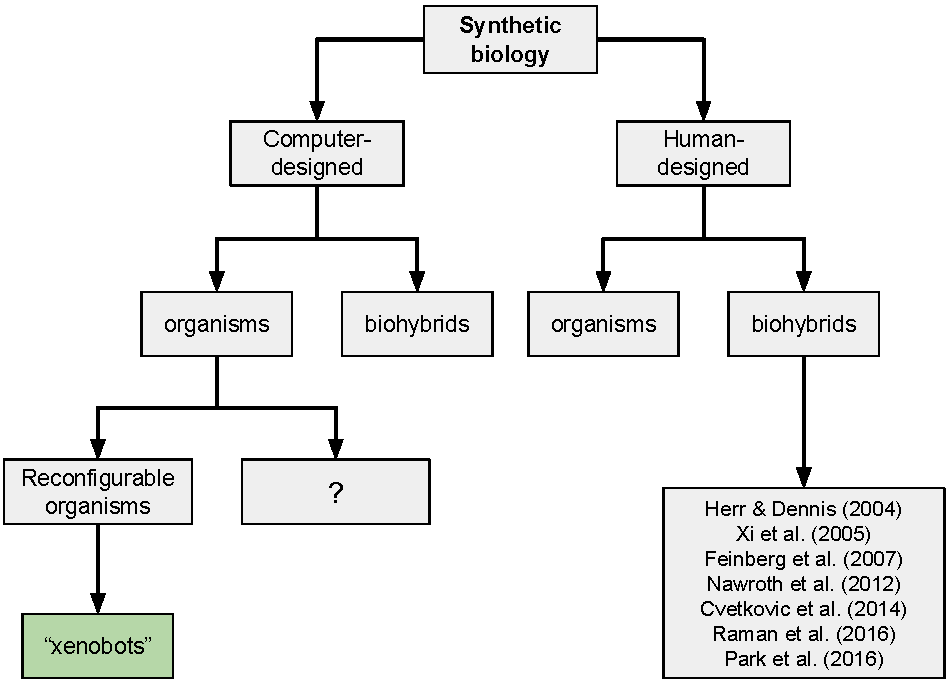
\includegraphics[width=\linewidth]{fig/synthbio.pdf}
    \vspace{1pt}
    \caption{%
    \textbf{Taxonomy of synthetic biology.}
    ``Where am I?'' --- a xenobot.
    \label{fig:synthbio}%
    }
\end{figure}




\section{Conclusion}

This thesis presented six sets of experiments (chapters 2, 3, 4, 5, 6 and 7), in which the morphologies of robots were permitted to vary on increasingly more scales in space and time.

